% Two side document:\documentclass[12pt,a4paper,twoside]{report}
% Open right: \documentclass[12pt,a4paper,twoside,openright]{report}
\documentclass[12pt,a4paper,twoside,openright]{report}
\usepackage[T1]{fontenc} % Standard package for selecting font encodings
\usepackage{mathptmx} % Use Times as default text font, and provide maths 
%support
\usepackage{amsmath,amssymb,amsfonts} % for math typesetting
\usepackage{setspace} % Set space between lines
\usepackage[top=1in,bottom=1in,left=3.2cm,right=2.6cm]{geometry} % page style 
\usepackage{graphicx}\graphicspath{{img/}} % for images 
\usepackage{subcaption} % for subfigures 
\usepackage[sort&compress]{natbib} % for references 
\renewcommand{\bibname}{References} % Rename Bibliography to References 
\usepackage[hidelinks]{hyperref} % for hyperlinks 

% Fancy Headers: Extensive control of page headers and footers in LaTeX
\usepackage{fancyhdr}\pagestyle{fancy} 
\fancyhf{}
\fancyhead[RE]{\it{\nouppercase{\leftmark}}}
\fancyhead[LO]{\it{\nouppercase{\rightmark}}}
\fancyhead[LE,RO]{\thepage}
\fancyfoot{}

\usepackage{emptypage}
\usepackage[nottoc]{tocbibind}
\setcounter{secnumdepth}{3}
\setcounter{tocdepth}{3}

% Title Page 
\title{Report Writing using \LaTeX\\[1.5cm] 
\includegraphics[scale=0.6]{latex}}
\author{Author Name}
\date{Institute Name\\ Department Name\\[5mm] \today}

\raggedbottom

\begin{document}

\pagestyle{empty}	

\maketitle	
\cleardoublepage

\onehalfspacing
\pagenumbering{roman}
\pagestyle{plain}

% Abstract 
\begin{abstract}
An abstract is a brief summary of a research article, thesis, review, conference proceeding, or any in-depth analysis of a particular subject and is often used to help the reader quickly ascertain the paper's purpose.
\end{abstract}	

% Clear Page
\cleardoublepage
% Set Page Style 
\pagestyle{fancy}

% Table of Contents, List of Figures, List of Tables 
\tableofcontents
\listoffigures
\listoftables	

\cleardoublepage
\doublespacing
\pagenumbering{arabic}	

% Import Chapters
% Chapter-1
\chapter{Introduction}\label{ch:ch1}
Lorem Ipsum is simply dummy text of the printing and typesetting industry. 
Lorem Ipsum has been the industry's standard dummy text ever since the 1500s, 
when an unknown printer took a galley of type and scrambled it to make a type 
specimen book. It has survived not only five centuries, but also the leap into 
electronic typesetting, remaining essentially unchanged. It was popularised in 
the 1960s with the release of Letraset sheets containing Lorem Ipsum passages, 
and more recently with desktop publishing software like Aldus PageMaker 
including versions of Lorem Ipsum.
Lorem Ipsum is simply dummy text of the printing and typesetting industry. 
Lorem Ipsum has been the industry's standard dummy text ever since the 1500s, 
when an unknown printer took a galley of type and scrambled it to make a type 
specimen book. It has survived not only five centuries, but also the leap into 
electronic typesetting, remaining essentially unchanged. It was popularised in 
the 1960s with the release of Letraset sheets containing Lorem Ipsum passages, 
and more recently with desktop publishing software like Aldus PageMaker 
including versions of Lorem Ipsum.. See figure~\ref{fig:im1}, \ref{fig:im2} of 
\ref{fig:subfigs cap}

Lorem Ipsum is simply dummy text of the printing and typesetting industry. 
Lorem Ipsum has been the industry's standard dummy text ever since the 1500s, 
when an unknown printer took a galley of type and scrambled it to make a type 
specimen book. It has survived not only five centuries, but also the leap into 
electronic typesetting, remaining essentially unchanged. It was popularised in 
the 1960s with the release of Letraset sheets containing Lorem Ipsum passages, 
and more recently with desktop publishing software like Aldus PageMaker 
including versions of Lorem Ipsum.

\section{Figures}
\begin{figure}
	\centering
	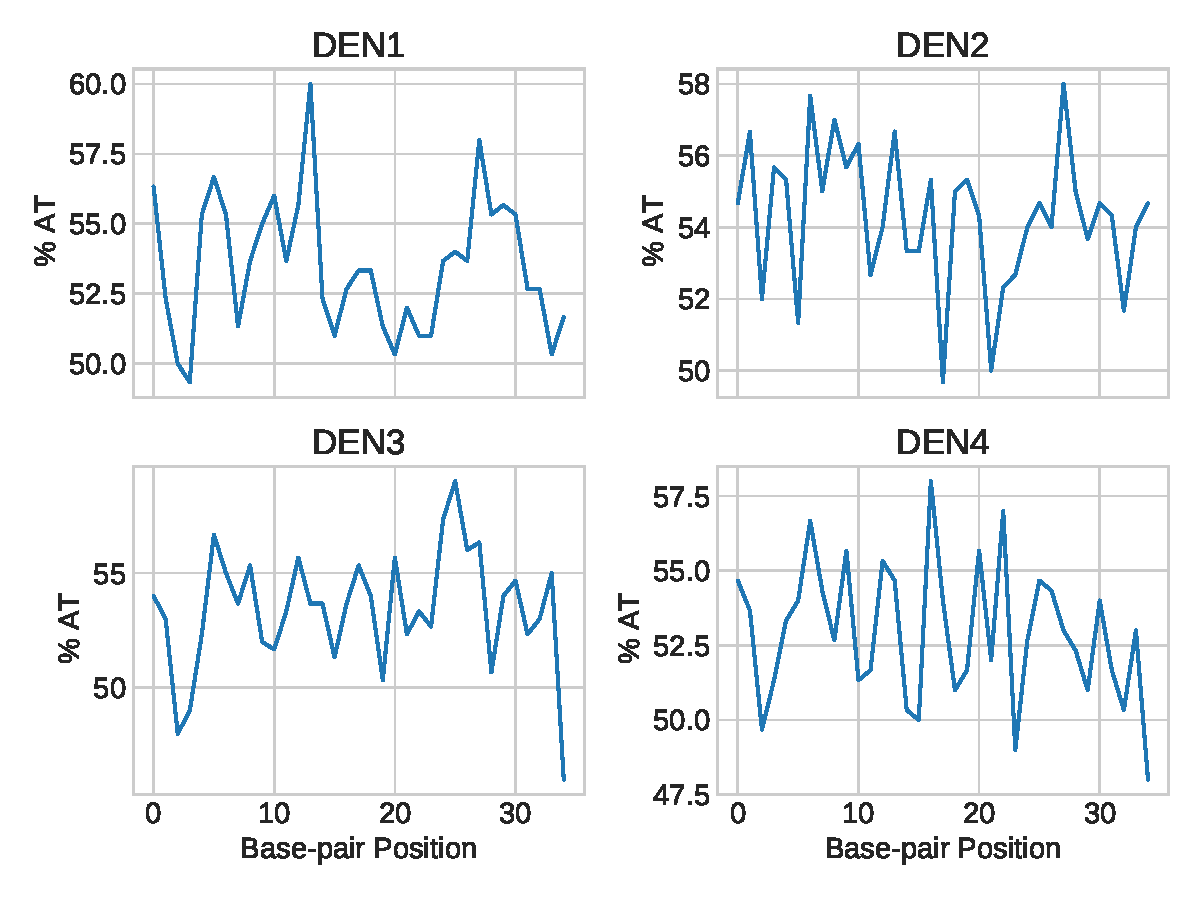
\includegraphics[width=0.7\linewidth]{den_plot}
	\caption{Caption of fig. 1.}
	\label{fig:image2}
\end{figure}

Lorem Ipsum is simply dummy text of the printing and typesetting industry. 
Lorem Ipsum has been the industry's standard dummy text ever since the 1500s, 
when an unknown printer took a galley of type and scrambled it to make a type 
specimen book. It has survived not only five centuries, but also the leap into 
electronic typesetting, remaining essentially unchanged. It was popularised in 
the 1960s with the release of Letraset sheets containing Lorem Ipsum passages, 
and more recently with desktop publishing software like Aldus PageMaker 
including versions of Lorem Ipsum.
\section{Subfigure}
Lorem Ipsum is simply dummy text of the printing and typesetting industry. 
Lorem Ipsum has been the industry's standard dummy text ever since the 1500s, 
when an unknown printer took a galley of type and scrambled it to make a type 
specimen book. It has survived not only five centuries, but also the leap into 
electronic typesetting, remaining essentially unchanged. It was popularised in 
the 1960s with the release of Letraset sheets containing Lorem Ipsum passages, 
and more recently with desktop publishing software like Aldus PageMaker 
including versions of Lorem Ipsum.

\begin{figure}
\centering
\begin{subfigure}[b]{0.45\textwidth}
  \centering
  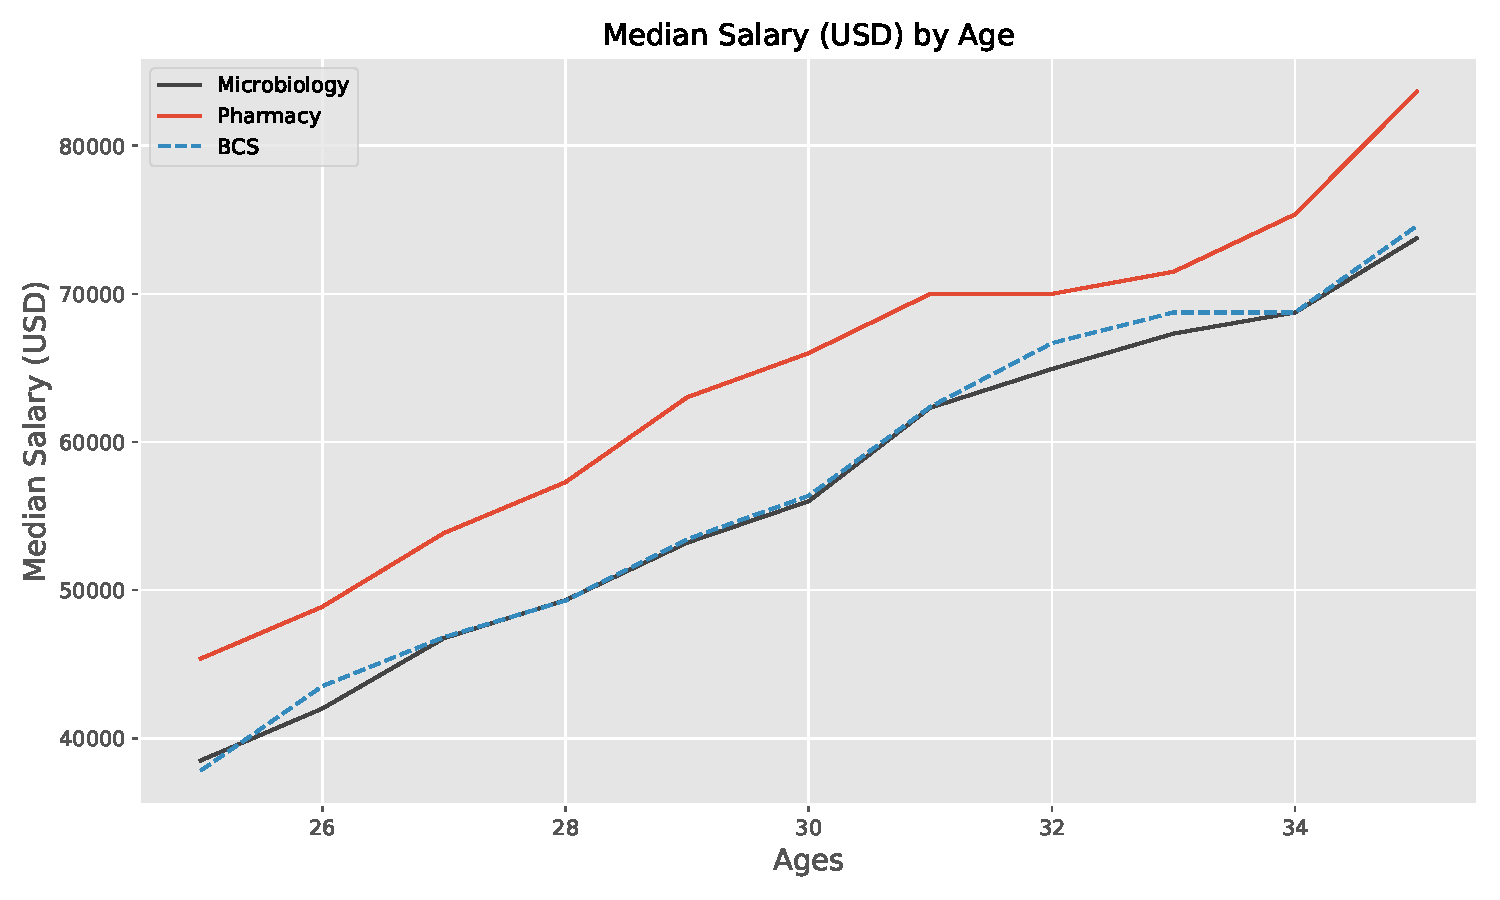
\includegraphics[width=\textwidth]{ggplot}
  \caption{}
  \label{fig:im1}
 \end{subfigure}
~
\begin{subfigure}[b]{0.45\textwidth}
  \centering
  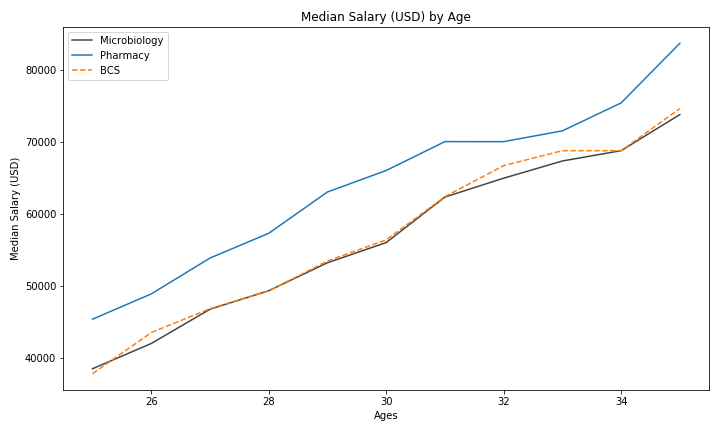
\includegraphics[width=\textwidth]{line}
  \caption{}
  \label{fig:im2}
\end{subfigure}
\caption{Two figure side by side}
\label{fig:subfigs cap}
\end{figure}

\section{Table}
Lorem Ipsum is simply dummy text of the printing and typesetting industry. 
Lorem Ipsum has been the industry's standard dummy text ever since the 1500s, 
when an unknown printer took a galley of type and scrambled it to make a type 
specimen book. It has survived not only five centuries, but also the leap into 
electronic typesetting, remaining essentially unchanged. It was popularised in 
the 1960s with the release of Letraset sheets containing Lorem Ipsum passages, 
and more recently with desktop publishing software like Aldus PageMaker 
including versions of Lorem Ipsum. Table~\ref{tab: sample}.

\begin{table}
\centering
\caption{Random table}
\label{tab: sample}
\begin{tabular}{|c|c|c|c|c|c|c|}
\hline 
1 & 2 & 3 & 4 & 2 & 3 & 4 \\ \hline 
5 & 6 & 7 & 8 & 2 & 3 & 4 \\ \hline 
9 & 10 & 11 & 12 & 2 & 3 & 4\\ \hline 
13 & 14 & 15 & 16 & 2 & 3 & 4\\ \hline 
\end{tabular} 
\end{table}
%================ch2======================================
\chapter{Genomic Data and Databases}\label{ch:ch2}

\section{What Are Genomic Data?}
Genomic data refers to the genome and DNA data of an organism. They are used in bioinformatics for collecting, storing and processing the genomes of living things. Genomic data generally require a large amount of storage and purpose-built software to analyze.


\section{Genomic Databases}
Genomic databases allow for the storing, sharing and comparison of data across research studies, across data types, across individuals and across organisms. These are not a new invention even before the popularisation of the modern internet, ‘online’ databases have been available in order to share data on key organisms, such as Escherichia coli (Blattner et al., 1997) and Saccharomyces cerevisiae (Cherry et al., 2012). Recent advances in both data sharing technology and genome sequencing technology have created an explosion of databases, based around particular organisms, as has been historically the case, as well as around particular data types, such as transcriptional data or short-read sequencing data\cite{gutierrez2019genome}. 

\section{Specific Organism Databases and the GMOD Project} 
It is possibly unsurprising that with the evolution of sequencing technology and the power to sequence the genome of most any organism, given a reasonable amount of time and a reasonable amount of research effort, individual databases have developed around the genomes of specific organisms \cite{ranganathan2018encyclopedia}. In the past, this was mostly focussed around so-called ‘model’ organisms, or ones with large research bases, such as the mouse (Mus musculus) (Smith et al., 2018) and nematode (Caenorhabditis elegans) (Lee et al., 2018).

In many cases, these were created by their own research communities, to suit their own needs, both in terms of how the data could be accessed, as well as what tools were provided to dissect the data. As efforts continued, there have been moves to create some consistency between databases and the tools they offer, meaning new organism databases are not required to ‘re-invent the wheel’ so to speak. In this regard, the Generic Model Organism Database (GMOD) project has served to provide a framework of tools and database methods to allow new databases to be created. The ‘users’ of the GMOD project are no longer limited to ‘model’ organisms, and now consist of a variety of different species and databases. The GMOD project also has its own genome browser associated with it, GBrowse (as discussed further below), which can be integrated into the participating databases as a web-based genome browser\cite{ranganathan2018encyclopedia}.


\section{Human Genome Databases}
The breadth and depth of human genome databases is vast, as is to be expected when an organism attempts to study itself, and
analyse its own biological problems. These databases are often structured around various data sources, such as transcriptional data,as is the case for the H-Invitational database (H-InvDB) (4). Particular study types have also given rise to specific databases:genome-wide association study databases such as GWASCentral (5), and structural variant study databases such as dbVar (6) and DGV (7). As is the case with other organisms, there are also some databases which seek to be more comprehensive in scope: DNA element databases such as ENCODE (8), and the 1000 Genomes project database, now hosted as the International Genome Sample Resource (IGSR) (9). Databases for even more specific purposes exist, such as a wealth of databases on cancer genomic data, and will need to be searched for on a case-by-case basis depending on need.


\section{The Main Three Databases}
The main three databases are the National Center for Biotechnology Information (NCBI, \url{www.ncbi.nlm.nih.gov/}), the DNA Data Bank of Japan (DDBJ, \url{www.ddbj.nig.ac.jp/}) and the European Bioinformatics Institute (EBI, \url{www.ebi.ac.uk/}). In addition to offering complete microbial genome sequences with links to corresponding publications, these databases provide online tools for analyzing genome sequences. As of February 24, 2014, 12 272 genome sequences from 2897 bacterial species are available online (www.genomesonline.org/, https://gold.jgi.doe.gov). For some species, several genomes have  been sequenced. For 31 species, more than 50 genomes areavailable,including 16 species for which more than 100 genomes have been sequenced, the species holding the record being Escherichia coli, with 1261 currently available genomes. Sequenced genomes include the most significant human bacterial pathogens, covering all the phylogenetic domains of bacteria. In addition, more than 27 000 sequencing projects are ongoing (  \url{www.genomesonline.org/})\cite{ray2003}. Moreover, new sequencing technologies are making possible the sequencing of random community DNA and single cells of bacteria without the need for cloning or cultivation. 

\section{Genome Browsers} 
Data access and quality means very little if no meaning can be gained from it. In a field with as complex and abstract data as
genomics, methods for data visualisation and analysis are of even greater importance. These must be able to cope with vast
amounts of data, in the order of gigabytes or terabytes, as well as be able to connect these to tangible, biological meaning in the form of genes and products. Genome browsers seek to fill this need by providing a pre-existing software basis to visualise and analyse genomic data. Due to the sheer variety of researchers, purposes, expectations, and goals involved in the field, a number of genome browsers are available. For the new user, there are three broad-class, easy-to-pick-up databases for generic uses that stand out at present: the UCSC Genome Browser, managed by the University of California, Santa Cruz (Casper et al., 2018); GBrowse, managed by the GMOD project (see “Relevant Website section”); and Ensembl, managed by EMBL-EBI and the Wellcome Trust Sanger Institute (Zerbino et al., 2018). This section will consider each of these browsers in turn, and then give an overview of the
more specific browsers which have been created based on these three forerunners\cite{ranganathan2018encyclopedia}.

\subsection{UCSC Genome Browser}
UCSC Genome Browser is the one of the most widely regarded broad-class browser, and has been integrated into a number of
major databases. Its initial conception in 2000 was to visualise the first working draft of the Human Genome Project, but has been adapted in the following years to include a broad variety of organisms, and a vast suite of tools for visualising and analysing data.(\url{https://genome.ucsc.edu/})

\subsection{Gbrowse} 
Due to the ‘generic’ nature of the GMOD project (discussed above at 2.2), there was a need for a generic browser to accompany the suite of tools provided for new databases. GBrowse developed from this idea, and is therefore one of the more flexible genome browsers available. It has had a number of spin-off browsers created since its conception, tailored for particular purposes. As it is a part of the GMOD project, it is also available across many different databases\cite{ranganathan2018encyclopedia}. (\url{http://gmod.org/wiki/GBrowse})

\subsection{Ensembl} 
The Ensembl genome browser created by EMBL-EBI and the Wellcome Trust Sanger Institute is the native genome browser for the
Ensembl Genomes databases. Due to the broad nature of the databases it is used for, it contains a broad variety of tools for visualisation and analysis across a variety of kingdoms of organisms.(\url{http://ensemblgenomes.org/})

\subsection{Specialised Browsers}
Browsers for more specialised purposes have been developed by particular groups, largely based on one of the primary three
browsers. Due to its generic nature, the majority of ‘subsidiary’ browsers are based on GBrowse in particular. Lighter implementations have been created, such as JBrowse, as well as browsers more suited to collaboration and annotation, such as Apollo.


	
%================ch3======================================
\chapter{Genomics Application}\label{ch:ch3}

\section{Role of Genomics in Clinical Microbiology} 
There are multiple applications for genomics in clinical
microbiology\cite{ray2003}. 
\begin{itemize}
	\item  Real-time genomics may be used to investigate infectious disease outbreaks
	\item  Bacterial genomes may be used as target sources for molecular detection, identification or genotyping.
	\item The gene content, obtained by comparison to databases such as Clusters of Orthologous Groups (\url{www.ncbi.nlm.nih.gov/COG/}) or Kyoto Encyclopedia of Genes and Genomes (\url{www.genome.ad.jp/kegg/}), may be searched for specific phenotypic traits such as virulence or antibiotic resistance markers, or deficient metabolic pathways enabling design of improved culture media.
	
	\item Antigenic epitopes detected in the deduced proteome may be
	used for serologic applications, development of monoclonal
	antibodies or development of vaccines (Figure~\ref{fig:genome}).
	\item Taxonomic description of new bacterial species.
\end{itemize}

\begin{figure}
	\centering
	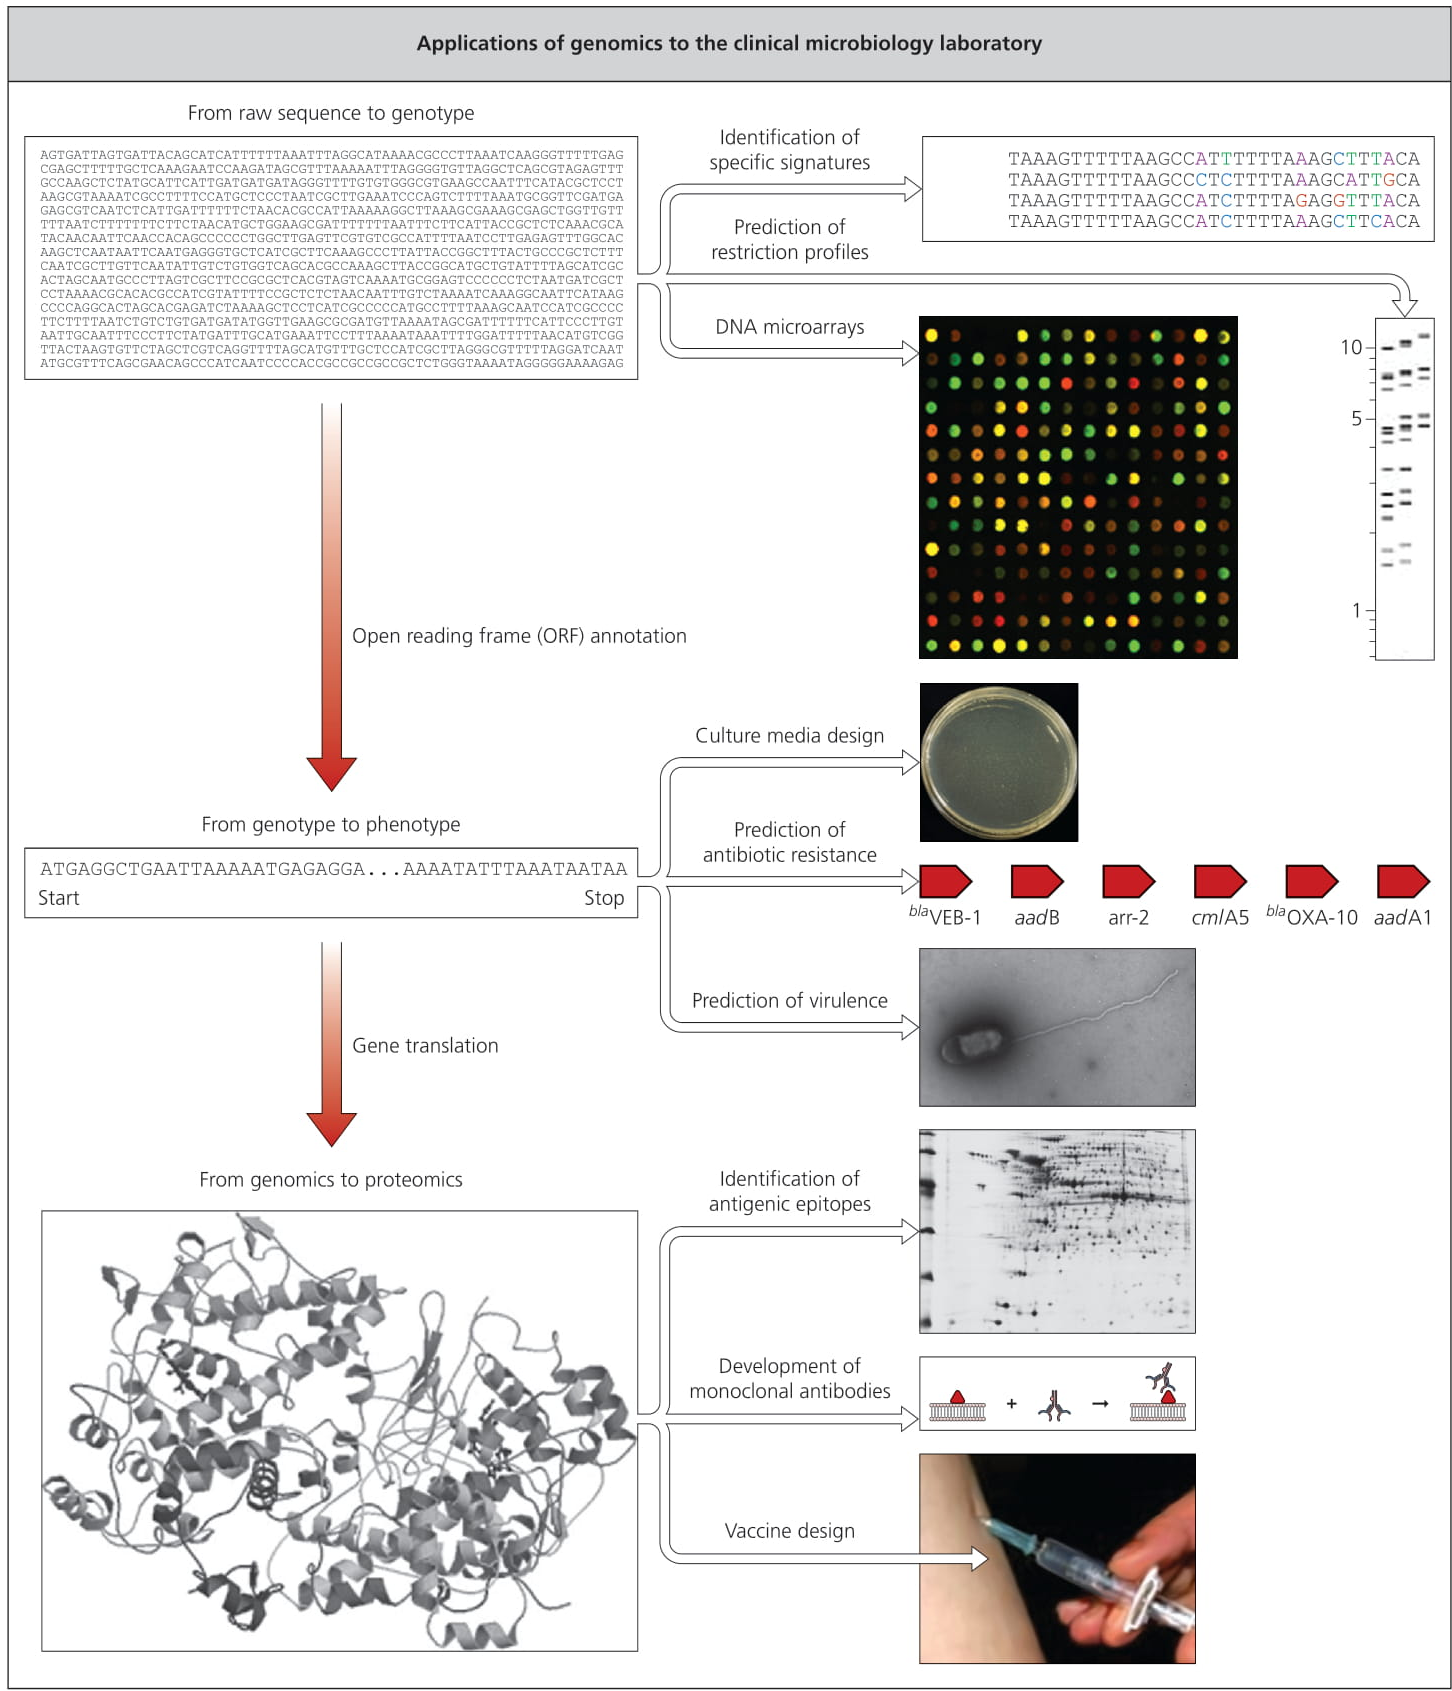
\includegraphics[width=0.9\linewidth]{backterial_genome}
	\caption{Applications of genomics to the clinical microbiology laboratory.}
	\label{fig:genome}
\end{figure} 


\section{The Clinical Applications of Genomic Technologies}
The clinical applications of genomic technologies are vast and offer opportunities to improve healthcare across the breadth of medical specialities. I will explore some of these applications in more depth this section.

\subsection{Gene discovery and diagnosis of rare monogenic disorders} 
Genomic technologies can be used by clinicians from all specialities to diagnose their patients who have high-risk genetic errors causing disease. Researchers are using these techniques to identify new genes which cause genetic disease at an astonishing rate - over 4000 diseases now have a known single genetic cause, compared to around 50 in 1990.

\subsection{Identification and diagnosis of genetic factors contributing to common disease} 
Genomic technologies are increasingly being used to understand the contribution of both rare and common genetic factors to the development of common diseases, such as high blood pressure, diabetes and cancer.

\subsection{Pharmacogenetics and targeted therapy}
Genetic information may be used to predict whether a person will respond to a particular drug, how well they will respond to that drug and whether they are likely to get any side effects from the use of a specific drug. This allows their treating team to make individualised decisions about the right drug treatment. In some cases, such as cancer, we can identify the genetic drivers of disease and then give drugs which specifically target that pathway. This is known as targeted therapy.

\subsection{Prenatal diagnosis and testing}
Genetic diseases are often devastating and may cause significant disability and even death in childhood. Prenatal diagnosis of genetic diseases allows parents to make decisions about whether to continue with the pregnancy or to allow early diagnosis and possible treatment in utero or at birth. Whilst previous approaches to prenatal diagnosis could put the pregnancy at risk, new methods using genomic technology can look directly at the DNA of the fetus from a maternal blood test, without increasing the risk of miscarriage - this is known as non-invasive prenatal testing. The use of NGS and array technology in prenatal samples is also on the increase to improve diagnostic yields in a pregnancy.

\subsection{Infectious diseases} 
Sequencing the genomes of microorganisms which cause human infection can identify the exact organism causing symptoms, help to trace the cause of infectious outbreaks, and give information as to which antibiotics are most likely to be effective in treatment.


\subsection{Personalised medicine}
As the exact DNA sequence of the genome of each human is unique to them, we will all have unique disease susceptibilities and treatment responses. Personalised medicine describes the use of our genetic information to tailor health care intervention to our own individual need.

\subsection{Gene therapy}
Gene therapy involves the administration of DNA or RNA, in order to correct a genetic abnormality, or modify the expression of genes.

\subsection{Genome editing}
Genome editing uses molecular techniques to modify the genome - genome editing can add in, cut out, or replace sections of the DNA sequence.

\subsection{Design of new antimicrobial agents and vaccines}
One of the expected benefits of genome analysis of pathogenic bacteria is in the area of human health, particularly in the design of more rapid diagnostic reagents and the development of new vaccines and antimicrobial agents. These goals have become more urgent with the continuing spread of antibiotic resistance in important human pathogens. Moreover, results from the whole-genome analysis of human pathogens has suggested that there are mechanisms for generating antigenic variation in proteins expressed on the cell surface that are encoded within the genomes of these organisms\cite{fraser2000microbial}.
These mechanisms include the following:

\begin{enumerate}
	\item slipped-strand mispairing
	within DNA sequence repeats found in 58-intergenic regions and coding sequences as described for \textit{H. influenzae2} \textit{ Helicobacter pylori26}  and \textit{M. tuberculosis27} 
	
	\item recombination between homologous genes
	encoding outer-surface proteins as described for Mycoplasma
	genitalium28, Mycoplasma pneumoniae29 and Treponema pallidum30 (Figure~\ref{fig:vac})
	
	\item clonal variability in surface-expressed proteins as described for Plasmodium falciparum31 and possibly Borrelia burgdorferi32. \cite{fraser2000microbial}
	
\end{enumerate} 

\begin{figure}
	\centering
	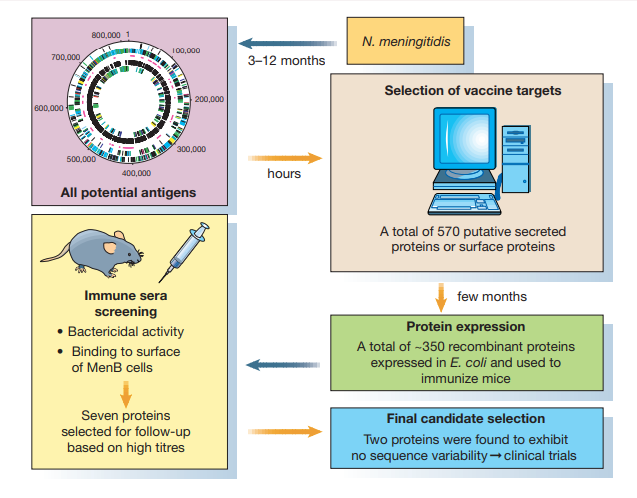
\includegraphics[width=0.9\linewidth]{vaccine}
	\caption{ Diagram depicting how complete microbial genome sequence data can accelerate vaccine development.}
	\label{fig:vac}
\end{figure} 

	

% Import Appendix 
\appendix	
%%
\chapter{Constants and Some Basic Units}

\section{Mathematical constants}
\begin{align*}
\pi = & \ 3.14159\ldots\\
e =  &\  2.1728\ldots\\
\ln10 =  & \  2.30259\ldots\\
\log10 =  &\  1
\end{align*}

\section{International System (SI) basic units}
\begin{table}[h]
	\centering
	\begin{tabular}{llll}
		\toprule[1.5pt]
		Quantity  &	Unit & Symbol & Dimension symbol\\
		\midrule[1pt]
		length & meter & m & L\\
		mass & kilogram & kg & M\\
		time & second & s & T\\
		electric current & ampere & A& I\\
		temperature & kelvin & K& $\theta$\\
		amount of substance & mole &   mol & N\\
		luminous intensity & candela & cd & J\\
		\bottomrule[1.5pt]
	\end{tabular}
\end{table}	

\singlespacing

% Import BibTeX
% Bibliographystyle: plain, abbrv, acm, 
\bibliographystyle{plain}	
\bibliography{references}
	
\end{document}